\section{Evidence-Guided Adaptation and Evaluation}\label{sec:protocol}
\subsection{Aligned Supervision Views}
For image $I_i$, question $q_i$, short answer $a_i$, and compact evidence $e_i$, the two principal targets are
\begin{equation}
y_i^A=a_i,\qquad y_i^E=\texttt{Evidence: }e_i\;\texttt{Answer: }a_i.
\label{eq:targets}
\end{equation}
The views retain identical record IDs, input questions, images, and final answers. Reference graphs, source-edit labels, typed results, and expected evidence are not appended to model inputs. Consequently, a difference between the two adapters concerns the tested supervision recipe, rather than access to additional inference-time annotations. Figure~\ref{fig:supervision} illustrates the input/output comparison. In the illustrated continuity-test case, either of two series-contact faults explains the failed observation. The compact certificate names both candidates and their shared observable consequence, exposing the distinction between fault compatibility and unique diagnosis. This supervision is intended to teach electrically relevant alternatives and the limits of available information, rather than only a binary label. Its utility is tested through answer correctness and evidence validity; improvement over answer-only training is not assumed.

\begin{figure*}[t]
\centering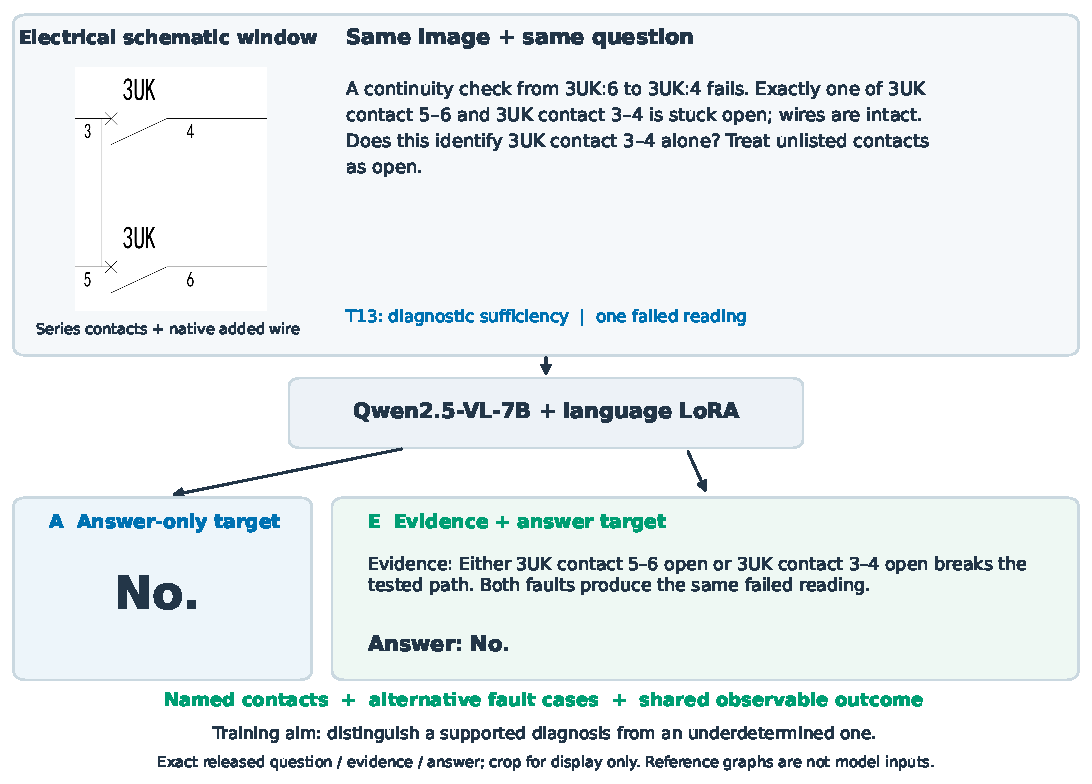
\includegraphics[width=\textwidth]{assets/figure_05.pdf}
\caption{Aligned supervision illustrated by a diagnostic-sufficiency example from the ELEC-VQA dataset. The same image and exact released question lead to either the short answer (A) or the released compact evidence followed by the same answer (E). The evidence identifies two distinct contact faults that produce the same failed continuity reading. Targets are reference annotations, not model predictions; the screenshot is cropped only for display. Equal examples and epochs do not imply equal token exposure or computation.}
\label{fig:supervision}
\end{figure*}

The backbone is Qwen2.5-VL-7B-Instruct~\cite{bai2025qwen}. Standard LoRA~\cite{hu2021lora} updates language attention query, key, value, and output projections; pretrained backbone and vision weights remain frozen. The assistant-token objective is
\begin{equation}
\mathcal L=-\sum_i\sum_{t\in\mathcal A_i}\log p_\theta(y_{i,t}\mid I_i,q_i,y_{i,<t}),
\label{eq:loss}
\end{equation}
where $\mathcal A_i$ excludes user, image, and padding positions. All assistant target tokens receive equal loss weight. Because the evidence target is longer, equal epochs do not imply equal supervised-token exposure or computation.

Fine-tuning uses BF16, rank 16, scaling 32, dropout 0.05, learning rate $10^{-4}$, three epochs, microbatch one, and gradient accumulation eight. Image area and context length are capped at 2,097,152 pixels and 8,192 tokens. The slow Qwen processor and scaled dot-product attention are fixed. Runs use Ubuntu 22.04 and one NVIDIA H100 GPU. The primary comparison uses seed 42 and the final-epoch adapters. Table~\ref{tab:training} summarizes the training settings.

\begin{table*}[t]
\centering\small
\caption{Matched training configuration for answer-only and compact-evidence fine-tuning.}
\label{tab:training}
\begin{tabularx}{\textwidth}{@{}XXX@{}}\toprule
Setting & Answer only & Evidence--answer \\\midrule
Backbone & Qwen2.5-VL-7B-Instruct & Qwen2.5-VL-7B-Instruct \\
Training QA / images & 6,972 / 697 & 6,972 / 697 \\
Target format & Short answer & Compact evidence, then answer \\
Adapted projections & Language $q,k,v,o$ & Language $q,k,v,o$ \\
LoRA rank / scaling / dropout & 16 / 32 / 0.05 & 16 / 32 / 0.05 \\
Precision / attention & BF16 / SDPA & BF16 / SDPA \\
Learning rate / schedule & $10^{-4}$ / cosine & $10^{-4}$ / cosine \\
Epochs & 3 & 3 \\
Microbatch / accumulation & 1 / 8 & 1 / 8 \\
Maximum pixels / context tokens & 2,097,152 / 8,192 & 2,097,152 / 8,192 \\
Processor / primary seed & Slow / 42 & Slow / 42 \\
Checkpoint policy & Final epoch & Final epoch \\
Updates / supervised tokens & \pending & \pending \\
\bottomrule\end{tabularx}
\end{table*}

\subsection{Reference-Guided Semantic Assessment}
Surface-form exact match is insufficient for comparing free-form baseline responses with adapters trained on concise targets. A correct decision need not begin with a fixed prefix, whereas an almost identical sentence can reverse a contact state or terminal relation. We therefore specify a common reference-guided judge, inspired by LAVE~\cite{manas2024lave}, for every compared model. Each request contains the exact question, the complete unmodified response, the reference short answer, a fixed task rubric, and a deterministic reference-fact package. The package includes typed results, relevant task parameters, labeled nodes and edges, and verification queries. These are evaluation-side annotations; the tested VQA model receives only its image and question. The judge is not asked to independently reinterpret the screenshot.

Ratings concern whether the final answer satisfies the electrical task, rather than resemblance to the reference wording. The task rubric preserves terminal identities, negation, explicit conditions, set completeness, and path order; alternative valid minimum plans or conducting routes are admissible. A solution that cannot be established from the reference specification remains unresolved. The same request construction and rubric apply to Base, A, E, and cross-family baselines. 

Let $r_i\in\{1,2,3,\bot\}$ be the judge rating, where 3 denotes a fully correct answer, 2 an explicitly correct but incomplete answer when permitted by the task rubric, 1 an incorrect or absent answer, and $\bot$ an unresolved evaluation. For resolved responses, the auxiliary semantic score is
\begin{equation}
s_i=(r_i-1)/2,\qquad c_i=\mathbb{1}[r_i=3].
\label{eq:judgescore}
\end{equation}
Only full credit contributes to the primary accuracy. Binary decisions, three-way state classification, and a single relation category do not receive partial credit. Evaluator uncertainty is not a score of $0.5$. With $\mathcal R$ the resolved subset of an $N$-question panel, unresolved evaluations give the reporting bounds
\begin{equation}
 A^-={\textstyle\sum_{i\in\mathcal R}c_i\over N},\qquad
 A^+=A^-+{N-|\mathcal R|\over N}.
\label{eq:unresolvedbounds}
\end{equation}
These bounds describe the original automatic-only sensitivity analysis; the provisional supplementary scoring in Section~\ref{sec:experiments} is reported separately. They are missing-judgment bounds, not statistical confidence intervals. Coverage is $|\mathcal R|/N$; mean semantic scores retain the same full-panel denominator and analogous bounds. Empty answers and clearly wrong decisions remain model failures, rather than being removed as unresolved cases.

Answer and evidence assessments are separated. Additional explanatory tokens neither earn answer credit nor incur a length penalty. A correct final answer with an invalid explanatory detail can receive answer credit but fails evidence or joint correctness; an unresolved contradiction in the final decision cannot be repaired by selecting its favorable sentence. Primary reporting uses QA-micro full-credit accuracy and equal-weight task macro accuracy over 14 families. T14's ten all-negative test questions are reported separately, leaving 2,064 questions in the primary held-out panel. Source-DWG macro accuracy and all-15-task results retain their explicit denominators. Reference quality and evaluator uncertainty limit the reliability of these automatic ratings~\cite{zheng2023judge,zeng2024llmbar}.

\subsection{Controlled-Change and Evidence Metrics}
Visual pairs use identical questions on different images, whereas condition pairs use the same image with a changed contact-state assumption. The pair audit checks question identity and reference outcomes, retaining both outcome-flip and invariant pairs.

For an admissible pair set $\mathcal P$, both responses must receive full credit; write $S_i=c_i$ for resolved judgments:
\begin{equation}
A_{\rm pair}=\frac{1}{|\mathcal P|}\sum_{(i,j)\in\mathcal P}S_i(\hat a_i)S_j(\hat a_j).
\label{eq:pair}
\end{equation}
An answer change alone does not establish successful change-sensitive reasoning: both predictions must satisfy their respective conditions. Pair statistics preserve the shared source identity and distinguish outcome-flip from invariant cases. The test inventory contains seven DWGs from two projects, limiting inferences about broader industrial populations.

Evidence is assessed for entity grounding, route or blocking-fact validity, compliance with stated conditions, treatment of necessary alternatives, and support for the answer. Joint correctness requires both a correct answer and valid evidence. Alternative valid certificates are accepted rather than matched verbatim. These criteria concern the observable explanation, not faithfulness to hidden computation~\cite{deyoung2020eraser,turpin2023unfaithful}.

\subsection{Common Inputs and Inference Budgets}
The controlled comparison contains the unchanged backbone (Base), the answer-only adapter (A), and the evidence--answer adapter (E). InternVL2\_5-8B and LLaVA-OneVision Qwen2 7B provide cross-family zero-shot context~\cite{internvl25card,llavaonevisioncard,li2024onevision}. Every comparator receives the same image and question under its native processor. Pixel budgets, tiling, visual tokens, checkpoint revisions, and prompts are logged; native processing is not described as pixel-identical preprocessing.

Two prompt tracks isolate answer ability from requested explanation. The main track appends ``Give a brief answer in English. Do not include an explanation.'' to the same released question for every comparator. A separate evidence-request track asks for relevant visible components, connections and conditions, followed by an \texttt{Answer:} line, for Base/A/E. Both tracks preserve the complete response for judging; the requested format is not a scoring criterion. Greedy decoding and a 768-new-token ceiling are checked on validation and frozen before test, with any truncation-driven revision documented. Text-only models supplied with netlists constitute a separate assisted-input condition, whereas text-only judges act solely on the evaluation side.